\documentclass[11pt]{standalone}


\usepackage{amssymb} 
\usepackage{amsmath} 

\usepackage[no-math]{fontspec}
\usepackage{unicode-math}
\setmainfont{Lato}
\setmathfont{Stix Two Math}

\usepackage{tikz}
\usetikzlibrary{arrows.meta}

\usepackage{xcolor}
\definecolor{itwm_blue_04}{HTML}{005A94}
\usepackage{nicefrac}


\begin{document}
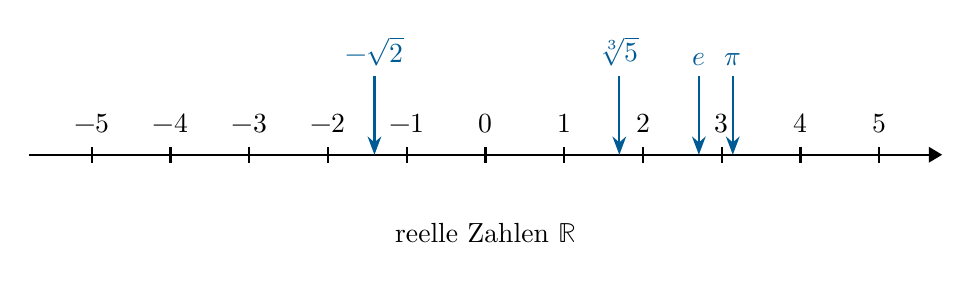
\begin{tikzpicture}
	\draw (0, -1) node {reelle Zahlen $\mathbb{R}$};
	\draw [-{Triangle}, thick] (-5.8,0) -- (5.8,0);
	\foreach \x in {-5,...,5} {
        \draw [thick] (\x,-.1) -- (\x,0.1);
        \draw (\x,0.4) node {$\x$};
    }
    \draw [itwm_blue_04, thick, -{Stealth}] (-1.41,1) node [above] {$-\sqrt{2}$} -- (-1.41,0);
    \draw [itwm_blue_04, thick, -{Stealth}] (1.7,1) node [above] {$\sqrt[3]{5}$} -- (1.7,0);
    \draw [itwm_blue_04, thick, -{Stealth}] (2.71,1) node [above] {$e$} -- (2.71,0);
    \draw [itwm_blue_04, thick, -{Stealth}] (3.141,1) node [above] {$\pi$} -- (3.141,0);
\end{tikzpicture}
\end{document}